% !TEX root = /Users/Gela/Desktop/Thesis_latex/thesis.tex

\section{Semi-permeable membrane}
\label{sec:membrane}
A membrane is defined as a barrier between two homogeneous phases. The process is a continuous steady-state operation consisting three streams: feed, permeate and reject. Main concern in the process boundary is the semipermeable barrier that selectively allows the passage of some components but not others. \cite{Singh}

\section{Osmosis} 
\label{sec:osmosis}
The osmosis process occurs when two solutions of different chemical concentration are separated by a semi-permeable membrane. The two different solutions will try to reach equilibrium. The solution with less concentration will have a natural tendency to migrate through the membrane over to the side with higher concentration.  
Osmosis is a naturally occurring phenomenon and one of the most important processes in nature. The pressure that occurs is called the osmotic pressure. The phenomenon can be seen in Figure \ref{fig:osmosis}. The fresh water on right side inte figure wants to contract through the semi-permeable membrane in order to reach a equilibrium with the salt water on the left side. This creates a stream of water from right side of the membrane to the left side. The osmotic pressure created by the different salute concentration in the fresh and salt water creates the flow. A greater difference in concentration creates a higher osmotic pressure than lower concentration difference.

\begin{figure}[h]
    \centering
    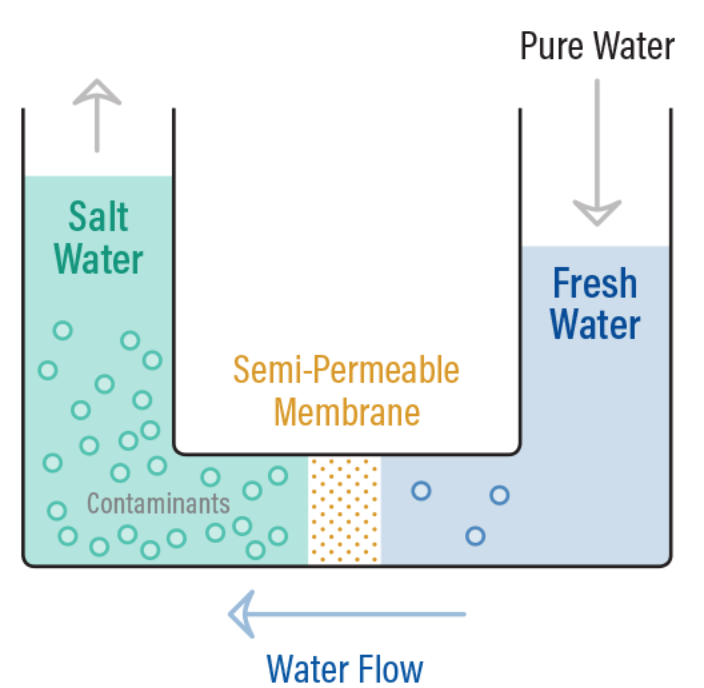
\includegraphics[width=0.4\textwidth]{Osmosis}
    \caption{Osmosis}
    \label{fig:osmosis}
\end{figure}

\section{Reverse osmosis}
\label{RO}
The reverse osmosis(RO) process is the reverse process of the osmosis. The idea is putting a pressure on the high concentration side in order to overcome the osmotic pressure, created by the difference in contaminant concentration. When pressure is applied to a semipermeable membrane, the water molecules are forced through the semipermeable membrane and the contaminants are not allowed true. The amount of pressure required depends on the salt concentration of the water. In order to gain reverse osmosis the pressure applied must be greater than the osmosis pressure. The membrane employs cross filtration rather than standard filtration. With cross filtration, the solution passes through the filter with two outlets. One solution passes true the membrane and is called permeate and is the filtered, pure, solution. The other solution can be drained or fed back into the filtering system, and is called reject. This can be seen in figure \ref{fig:ROsystem}. \\
\\
The contaminants build up att the surface area and it is of great importance to try to sweep them away and hold the surface clean. If the contaminants builds up the performance of the membrane will decrease, and cleaning with chemicals or heat water might be necessary \cite{Puretech}. The phenomenon of reverse osmosis can be seen in \ref{fig:ReverseOsmosis}. The water on left side is pressured through the membrane to the right side since the applied pressure is higher than the osmotic pressure. The result is a pure water with only small amount of contaminants in the fresh water stream. 
\begin{figure}[h]
    \centering
    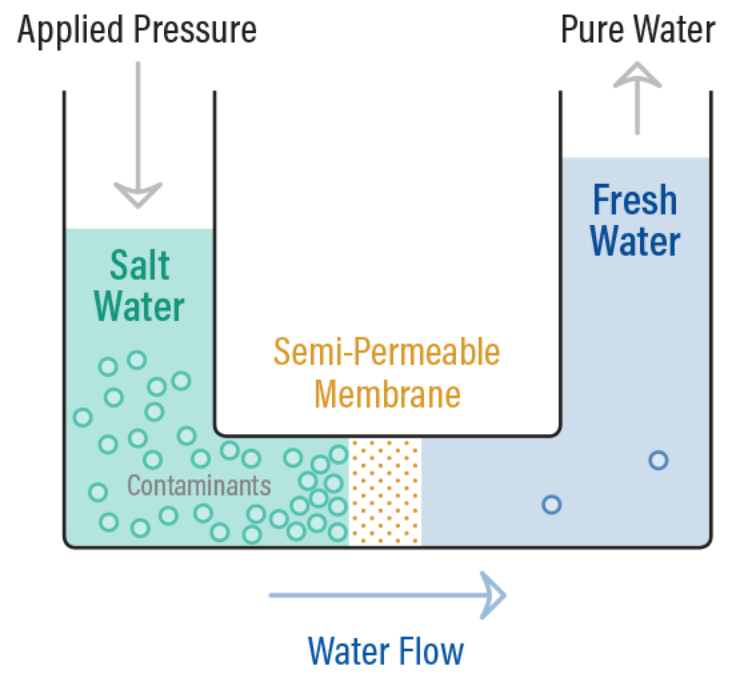
\includegraphics[width=0.4\textwidth]{ReverseOsmosis}
    \caption{Reverse Osmosis}
    \label{fig:ReverseOsmosis}
\end{figure}

\begin{figure}[h]
    \centering
    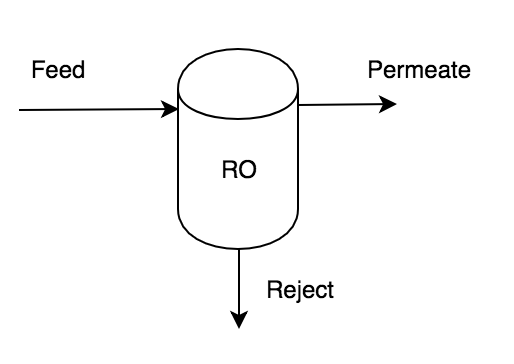
\includegraphics[width=0.4\textwidth]{ROsystem}
    \caption{RO-system}
    \label{fig:ROsystem}
\end{figure}


%In order to obtain good performace over the RO membrane there are some parameters that should be taken in consideration when designing a RO system. These are:

%\begin{labeling}{alligator}
%\renewcommand\labelitemi{ }
%\item [Pressure:]  feed ($P_{f}$), permeate ($P_{p}$), reject, ($P_{r}$)
%\item [Conductivity:] feed, $C_{f}$, permeate ($C_{p}$), reject ($C_{r}$)
%\item [Flow:] feed ($Q_{f}$), permeate ($Q_{p}$), reject($Q_{r}$)
%\item [Temperature:] feed ($T_{f}$), permeate ($T_{p}$), reject ($T_{r}$)
%\end{labeling}


\subsection{Fouling}
Fouling occurs when contaminants accumulate on the surface of the membrane on feed to reject side. The fouling contributes to a pressure drop that will decrease the performance of the membrane and cause less permeate(fresh water) flow. Fouling will happen eventually to some extent given the fine pore size of the membrane. A high reject flow and proper pretreatment will extend the operational time between cleaning procedures of the membrane \cite{Puretech}. 

\section{Mathematical modeling of reverse osmosis} 
\label{sec:soldiff}
There are different models to describe the flow of solutes and solvents in the reverse osmosis process. The mass balance equations are central in modeling the process. Figure \ref{fig:ReverseOsmosis} shows the main process. The mass balance equations is applied to feed, permeate and reject side, as in figure \ref{fig:ROsystem}. \\
\\
A hydraulic pressure is applied to to the feed stream of concentration, $C_{f}$ and results in a flow rate $Q_{f}$. Some of the solvent, pure water, passes through the RO-membrane characterized by solvent permeability, solute permeability and surface area. The product water (purified water), is called permeate and has the concentration $C_p$ and flow $Q_p$. The concentration, called reject has the concentration $C_r$ with flow $Q_r$. The study objective of this basic RO-modeling is to calculate output concentrations and flow rates in terms of input and operation conditions. Parameters used to evaluate the performance of the RO-membrane is rejection ratio:
\begin{equation}
\label{eq:rejection}
R=1-\frac{C_{p}}{C_{f}}
\end{equation}
and recovery ratio:

\begin{equation}
\label{eq:recovery}
Y=\frac{Q_{p}}{Q_{f}}
\end{equation}
which express the quality and quantity of the solvent product respectively. 
\\Mass balance in the system gives:

\begin{equation}
\label{eq:feedflow}
Q_{f}=Q_{p}+Q_{r}
\end{equation}
and:

\begin{equation}
\label{eq:mass}
C_{f}Q_{f}=C_{p}Q_{p}+C_{r}Q_{r}
\end{equation}
Solvent flux per unit time per unit membrane surface area is described by:

\begin{equation}
\label{eq:flux}
J_{w}=\frac{Q_{p}}{A_{m}}= A(\Delta P - \Delta \pi)
\end{equation}
where $\Delta\pi = \pi_{f} - \pi_{p}$ is the osmotic pressure difference between feed and permeate side and $A_{m}$ is membrane surface area.
Solute flux is given by:

\begin{equation}
\label{eq:solflux}
J_{s}=B(C_{f}- C_{p})
\end{equation}
 where B is the solute permeability.
\\The permeate concentration can be described by:

\begin{equation}
\label{eq:permcond}
C_{p}=\frac{C_{f}}{1+\frac{A}{B}(\Delta P - \Delta\pi)}
\end{equation}
where A is solvent permeability.
Permeate flow is described by:

\begin{equation}
\label{eq:permflow}
Q_{p}=Q_{f}Y
\end{equation}

The four mass balance equations (\ref{eq:feedflow} - \ref{eq:solflux}) make the RO process mathematically solvable.

In order to model the osmotic pressure the van't Hoff principle can be used. It gives the osmotic pressure:
\begin{equation}
\label{eq:posm}
\Delta\pi=b(C_{f}-C_{p})
\end{equation}
where b is a proportionality. In van't Hoff's equation b=RT, where R is the gas constant and T is the absolute temperature om the membrane system. 

\subsection{Equations from DOW}
\label{sec:doweq}
%\newcommand{\mathleft}{\@fleqntrue\@mathmargin0pt}
\mathleft

\begin{equation}
\label{eq:pQ}
Q_{p}=A_{i}\pi_{i} S_{E}(TCF)(FF)(P_{fi}-\frac{\Delta P_{fcj}}{2}-P_{pi}-\pi+\pi_{p})
\end{equation}

%\begin{equation}
%\label{eq:avOsmP}
 %\pi_{i}= \pi_{fi} (\frac{C_{fci}}{C_{fi}})(pf_{i})
%\end{equation}

%\begin{equation}
%\label{eq:avOsmp2}
%\pi_{i}= \pi_{fi}(1-R_{i})
%\end{equation}

\begin{equation}
\label{eq:feedOsmP}
\pi_{f}= 1.12(273+T) \sum m_{j}
\end{equation}

\begin{equation}
\label{eq:TCF}
TCF =
\begin{cases}
e^{2640(\frac{1}{298}- \frac{1}{273+T})} , T\geq25 \\
e^{3020(\frac{1}{298}- \frac{1}{273+T})} , T\leq25
\end{cases}
\end{equation}

\begin{equation}
\label{eq:polfac}
pf_{i} = e^{0.7Y_{i}}
\end{equation}

\begin{equation}
\label{eq:recov}
Y= \frac{Q_{p}}{Q{f}}
\end{equation}

\begin{equation}
\label{eq:permC}
C_{p}=B(C_{fc})({pf_{i}})(TCF)\frac{S_{E}}{Q_{i}}
\end{equation}

\begin{equation}
\label{eq:permability}
A(\pi) =
\begin{cases} 
0.125 , \pi \leq 25 \\
0.125-0.011(\frac{\pi - 25}{35}) , 25 \leq \pi \leq 200 \\ 
0.07-0.0001(\pi-200) , 200 \leq \pi \leq 400  
\end{cases}
\end{equation}

\section{Control theory}
Control theory deals with the behaviour of dynamical systems. The inputs and outputs may vary in numbers, and the reference signal, output is controlled by manipulating the input signal to obtain the desired output of the system. The characteristics of the systems aims for different types of controlling. There exists different control methods to meet the differences in the characteristics of the systems. The control theory is basically split in two, linear and non-linear. In order to design a controller that is capable of regulating the system parameters as speed, linearity/non-linearity, complexity and robustness needs to be analysed before a specific method is chosen. Below, some key words and different types of control principles are presented. \\
\\
\textbf{Step-response:} The time behaviour of the outputs of a general system when the input is changed from zero to one in a very short time. \\
\textbf{Rise Time:} The time it takes for the plant output to rise beyond 90 \% of the desired level for the first time\\
\textbf{Overshoot:} How much the peak level is higher than the steady state, normalized against the steady state.\\ \textbf{Settling time:} The time it takes for the system to converge to steady state.\\
\textbf{Steady-state error:} the difference between the steady-state output and the desired output.\\
\textbf{Transfer function:} Gives the system output for each possible input.\\

%\subsection{Linear Quadratic Gaussian control (LQG)}
%Linear Quadratic Gaussian is considered being a combination of a Kalman filter, linear quadratic estimator (LQE) with a linear quadratic regulator (LQR). The method is called LQG since the regulator is linear, works with quadratic criterias and the noise is normally distributed, Gaussian. LQG control applies to both linear time-invariant systems as well as linear time-varying systems. The controller is a dynamic system and often has the same state dimensions as the system it is controlling. The optimum problem is separable in two independent parts: to calculate the optimum estimated states, the kalman filter, and to calculate the optimum feedback from the estimated states. Below describes briefly how a LQG controller is designed for a continuous system. The system can be displayed as:

%\begin{equation}
%\label{eq:LQG1}
%\begin{array}{lcl}
%\dot x(t) = A(t)x(t) + B(t)u(t) + v(t) \\ y(t) = C(t)x(t) + w(t)
%\end{array}
%\end{equation}
%where x(t) represents the vector of state variables in the system, u(t) the vector of control inputs and y(t) the vector of measured outputs available for feedback. The v(t) is white Gaussian system noise and the w(t) is white Gaussian measurement noise, both affecting the system. If searching for the 
%\begin{equation}
%\label{eq:LQG2}
%u(t) = - F_{y}(p)y(t)
%\end{equation}
%that minimize
%\begin{equation}
%\label{eq:LQG3} 
%V= \| z \| ^{2}_{Q_{1}} + \| u \| ^{2}_{Q_{2}}
%\end{equation} 
%for a positive definit matrice $ Q_{2} $ and a positive semi definit matrice $ Q_{1} $. The regulator is assumed causal. The optimum linear controller is:
%\begin{equation}
%\label{eq:LQG4}
%\begin{array}{lcl}
%u(t) =  -L \hat{x}(t) \\  \hat{\dot x} = A\hat{x} + Bu(t) + K(y(t)-C\hat{x}(t)) 
%\end{array}
%\end{equation}



\subsection{PID control}
The PID controller is the most commonly used algorithm for process control. 
PID control consists of three basic coefficients, P (proportional), I (integral) and D (derivative) which are varied to recieve a optimal system response. It has a robust performance in a wide range of operating conditions. The parameters needs tuning in order to giva an ideal response.\\
\\
The basic idea behind a PID controller is to read a signal from a sensor, compute the desired actuator output by calculate the P,I and D response and sum them to compute the output of the controller. The controller needs a given set point and a measured process value from the system. A closed loop system provides feedback to the control system and the offset between the set point and the measured value is compensated with the controller.
\\
\\
To achieve good performance of the controller the requirements of the system needs to be identified. The control system performance can be measured by applying a step function as the set point command variable, and then measure the response of the process variable.
\\
\\
\paragraph{Proportional component (P)} 
The proportional component (P) depends on the difference between the set point and the process variable. The difference between them is referred as the Error. The proportional gain determines the ratio of output response to the error signal. Increasing the proportional gain increases the speed of the control system response. If the gain is set to high an oscillation system behaviour is expected and the system will become unstable if the proportional gain is set too high. 
\\
\\
\paragraph{Integral component (I)}
The integral component (I) sums the error over time. A small error term will cause the integral component to increase slowly. The response will continuously increase over time as long as the error is not zero. A windup phenomenon may occur if the Steady-State error never reaches zero and an implementation of an anti-windup is often needed. If an anti-windup system is not implemented the controller keeps increasing the integral component without the controller driving the error signal towards zero. 
\\
\\
\paragraph{Derivative component (D)}
The derivative component (D) causes the output to decrease if the process variable increases rapidly. The response is proportional to the rate of change of the process variable. Increasing the derivative time parameter will cause the control system to react more strongly to changes in the error term and will increase the overall control system response. \cite{PID}
\\
\\
\subsection{Windup and methods to avoid it}
Windup occurs when the steady-state error never reaches zero and the integrating component increases and saturates the control signal. Below, two different ways of implementing anti-windup, conditional integration and Back-calculating, to avoid wind-up is presented.\\
\\
\paragraph{Conditional Integration}
Conditional Integration is an anti-windup method that stops the integration process when the output has reached a saturation limit. The method ensures that while the controller is experiencing saturation there is no further increase in the value of the output. When or if the the error reduces below certain level, making the output come out of saturation level, the integrator start again \cite{clamping}.
\paragraph{Back-calculating}
Back-calculating is a method that uses a PID controller on parallell form with a back-calculation factor calculated from a model of the actuator model. The back-calculating method uses one parameter to calculate if the output signal has saturate and limits the integrating part until saturation is no longer experienced. \cite{clamping}. \\
\\
\subsection{Tuning}
The process of setting the optimal gains for the P,I and D component is called tuning. The components shall be designed in order to get an ideal response from the system. There are many concepts on how to tune a PID-controller. Some is presented below.\\
\\
\paragraph{Ziegler-Nichols method}
The Ziegler-nochols method is a popular method of tuning a PID controller and conducts proposed rules for determining values of the gain (K) as: $K_{P}, K_{I} and K_{D}$ based on the transient step response of a plant. The relationship between $K_{P}, K_{I} and K_{D}$ are important and when tuning the system some rules of thumb can be used: \\
\\
- Adjust $K_{P}$ to decrease the rise time.\\
- Adjust $K_{I}$ to eliminate steady-state error.\\
- Adjust $K_{D}$ to reduce overshoot and settling time.\\
\\
Ziegler-Nichols tuning method is considered good as a initial tuning for PID-control for unknown systems. For the design of the gain parameter there are some guidelines to be followed:\\
Use a closed loop system with a proportional controller, $K_{P}$. Start with a low value of the gain, $K_{P}$, increase until a steady-state oscillation occurs and note the value as $K_{cr}$. 
The parameters $K_{P}, T_{i} and T_{d}$ can be estimated with this help parameter, $K_{cr}$ and $P_{cr}$ which is the period time(s) of the oscillations, as follows: $K_{P}= 0.6K_{cr}$, $T_{i}= 0.5P_{cr}$, $T_{d}= 0.125P_{cr}$ \ref{Z-N}. 
\\
\\
\paragraph{Lambda method for tuning PI controllers}
Lambda tuning is an approximative pole placement method. The tuning method has the potential to be a simple straight forward tuning method. The theory of the Lambda method is based on two assumptions. The first one where the process is modeled as a first order process with dead time. The second one where the closed loop transfer function is specified as:\\
\\
\begin{equation}
\label{eq:lambda}
G_{cl}(s) = \frac{e^{-sL}}{1+ sT_{cl}}
\end{equation}
where $ T_{cl} $ is the time constant of the closed loop, T is the time constant and L is the time delay.\\
\\
The lambda method can be used with cancellation of system pole for stable processes and without cancellation of system pole for stable or unstable processes. The lambda method requires only one tuning parameter, $ T_{cl} $ that is the desired closed loop constant. The choice of $ T_{cl} $ is a key decision in order to get a well performed system. $ T_{cl} $ can be choosed to any value, but in practice, an arbitrary choice can lead to poor performance or even instability, since the simple process models are only valid in certain frequency regions. Therefore the closed loop constant shall be related to the process dynamics, e.g. time constant(T) and time delay(L). To obtain a fast response with good rejection of disturbances it is desirable ta have a small value of $ T_{cl} $. A large value of $ T_{cl} $  gives a system that is more insensitive to parameter variations. \\
\\
If there is limited knowledge about the system dynamics it would be appropriate to use a relatively high value of $ T_{cl}  =T\lambda $ , where $\lambda$ is the adjustable parameter. If the system is considered having a little deadtime, a relatively small $ T_{cl} $ is appropriate. The $ T_{cl} $ can be determined by $ L\lambda $ in integrating processes. 
\cite{lambda}










